
\vspace{1cm}
\section{État de l'art}

\subsection{Introduction}

La mise en place d'un générateur du code automatique d’après une Modélisation DOMIS nécessite une grande étude sur tout existant dans ce domaine de modélisation, Présisement le concept B-ADSC sur lequel se base DOMIS ainsi que l'étude et l'analyse de ce dernier.


\subsection{Modélisation des systèmes Complexes}

B-ADSc : "Bucki – Analyse décisionnelle des Systèmes complexes" est une méthode dédiée à la conception et à l’analyse des systèmes et des organisations. Elle se distingue par la prise en compte effective des opérateurs humains avec leurs autonomies, leurs politiques de production, leurs procédés de prise de décision, leur retour d’expérience...

Dans la conception du Système d'Information, les flux des données et des traitements sont soumis aux flux des décisions : en cela B-ADSc généralise les analyses fonctionnelles. Ainsi, le Système d’information est intimement lié à l’Organisation des acteurs (hommes, machines) jusqu'à se confondre.

Conçue dans les années 1990 par Janusz Bucki \cite{B-ADSC}, docteur en mathématiques et ingénieur automaticien, alors qu’il conduisait des réalisations dans le domaine de l’industrie et de la défense en particulier pour la conception des systèmes à risque et à Intelligence distribuée, cette approche s’est étendue depuis au tertiaire, au monde de l'Internet - Internet des objets - et donne lieu à un enseignement.

Selon cette approche systémique, la caractéristique la plus importante de toute organisation est sa capacité à élaborer des Décisions relatives au pilotage des processus : elle s'attache donc à modéliser et à analyser les organisations selon l'ordonnancement des Décisions et non selon l'agencement des Fonctions...

Pour B-ADSc, une organisation correspond à une hiérarchie opérationnelle d’activités dans laquelle chaque activité représente un «centre élémentaire de prise de décision» pouvant être piloté par un homme ou par une machine.\cite{badsc}


\subsection{ Le concept d’activité}

En Analyse fonctionnelle, l’accent est mis sur les données (schémas de données) et leur transformation ou traitement (schémas des traitements). Ainsi, l’objectif de l’analyste serait plutôt de mettre en exergue le « comment » du système (voir schéma ci-dessous) et pas forcément le « pourquoi de ce comment ».

\begin{figure}[H]
\begin{center}
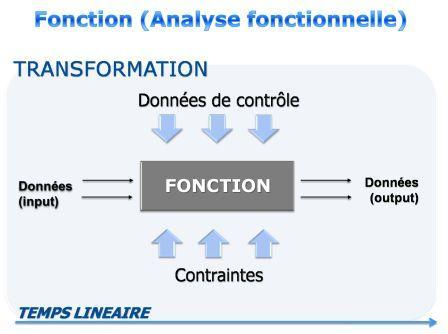
\includegraphics[width=0.5\linewidth]{images/analyse_fonctionnelle}
\end{center}
\caption{L'analyse fonctionnelle}
\label{fig:9}
\end{figure}

Ici, la fonction est comparable à une boîte noire. Elle peut être décomposée en sous-boîtes noires, l'organisation de ces boîtes n'ayant pas pour but de refléter l'organisation des acteurs. En automatisation, la notion de boucle de régulation permet d’adjoindre un « retour » (ou feedback) afin de passer du traitement à la régulation. La fonction peut donc, selon l’évolution du processus, être régulée.

B-ADSc positionne systématiquement le "Comment" dans le contexte de son "Pourquoi" et fait passer du "traitement des données" au "pilotage/régulation des situations" : piloter/gérer un processus signifie décider et contrôler son évolution afin de l’amener à une situation concordant avec les objectifs poursuivis.
La compréhension et l'interprétation des évolutions du processus s’opèrent dans le contexte des buts du décideur, exemple:
Evolution du processus : "je suis chez moi et il commence à pleuvoir"...
si mon but initial est d’arroser le jardin alors - c’est bon – "la nature s’en charge"si mon but est d’aller au théâtre alors - c’est mauvais - "risque d’être mouillé".

Les objectifs et le processus évoluant, le pilotage doit être perpétuellement réadapté : les écarts entre objectifs et réalité doivent diminuer ou, à minima, s’inscrire dans un seuil de tolérance (qui permet d’amener la situation – le processus – au plus près des objectifs poursuivis).
B-ADSc place ici l'activité à l’intersection de deux boucles de régulation qui prennent en compte l’évolution du processus (le comment) et celle des objectifs (le pourquoi).
 
 \begin{figure}[H]
\begin{center}
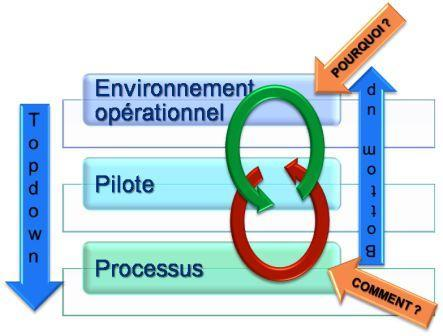
\includegraphics[width=0.5\linewidth]{images/comment_pourquoi}
\end{center}
\caption{L'intersection des deux boucles de régulation le comment et le pourquoi}
\label{fig:10}
\end{figure}
La « brique » de base de B-ADSc est une Activité. Elle est régulée (ou pilotée) par les activités de niveau supérieur qui lui délèguent des objectifs et régule (ou pilote) les activités de niveau inférieur qui constituent son processus.
Ainsi, elle encapsule deux fonctions
(voir schéma ci-dessous):

• « Fd » pour « Fonction décision » 

• « Fe » pour « Fonction évaluation » 

Une activité dispose nécessairement de quatre mémoires distinctes :

1.La mémoire des objectifs assignés par le niveau opérationnel supérieur 

2.La mémoire de l'état du processus piloté 

3.La mémoire des buts des décisions prises par l’activité 

4.La mémoire des changements d’état du processus

 
 \begin{figure}[H]
\begin{center}
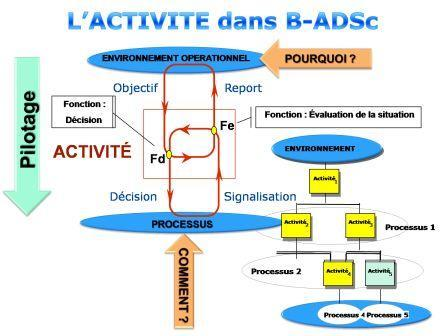
\includegraphics[width=1\linewidth]{images/activite}
\end{center}
\caption{L'activité dans B-ADSc}
\label{fig:11}
\end{figure}

 
B-ADSc interprète systématiquement le comportement d’une activité – prise des décisions, évaluation du processus - dans le contexte des objectifs poursuivis :
Je suis chez moi (« Je » = activité) et il pleut dehors (le « comment » du processus).

• Si mon but initial est d’arroser le jardin alors « c’est bon pour moi » (la nature fera à ma place, je n'ai rien à décider sauf annuler l'arrosage) 

• Si mon but est d’aller au théâtre alors « c’est mauvais pour moi » (je risque d’y arriver mouillé, je décide donc d'annuler ou de prendre un parapluie).\cite{badsc} 
